\subsection{FeatureSpy概览}
\label{subsec:featurespy-secure_design}

基于明文的攻击检测方案的一个安全缺陷是攻击检测程序容易被绕过(图~\ref{fig:featurespy-architecture-strawman-bypass})。具体来说,恶意客户端可以直接注入其自行构建的数据块执行未受保护的操作(例如,密钥生成等)处理,进而发起推测内容攻击(\S\ref{sec:background-enc-deduplication})。

\begin{figure}[!htb]
    \centering
    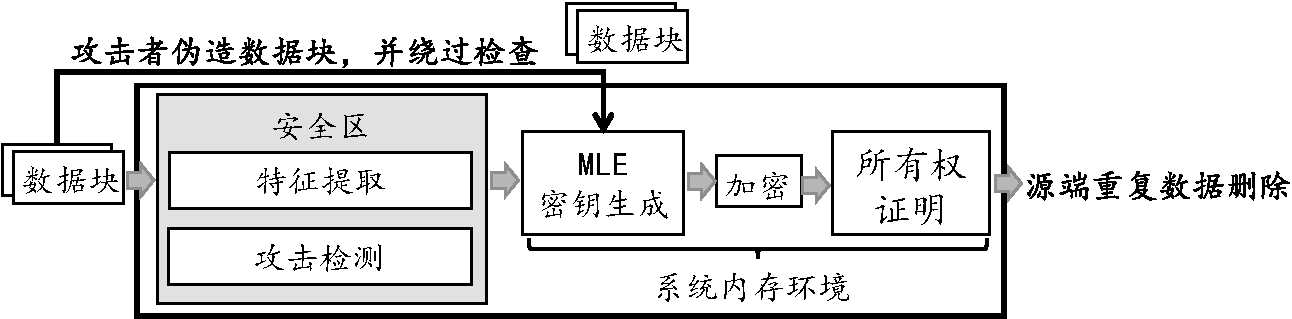
\includegraphics[width=\textwidth]{pic/featurespy/naive-problem.pdf}
    \caption{攻击检测程序被绕过}
    \label{fig:featurespy-architecture-strawman-bypass}
\end{figure}


\sysnameF 基于TEE的所有权证明方案(参见\S\ref{subsec:sgxdedup-arch})构建,以防止客户端绕过检测程序。具体来说,基于TEE的所有权证明方案将每个密文数据块作为输入并在安全区内计算密文数据块的指纹以及指纹对应的签名。进行重复数据删除时,云服务端在验证指纹对应的签名有效后才继续检查指纹是否对应于已存储的密文数据块(即发生重复数据删除)。由于云服务端仅响应具有签名的指纹,因此客户端无法对未签名的数据块进行重复数据删除查询(绕过攻击检测)。

因此,一种直接的方法是在基于明文的攻击检测方案中扩大安全区大小,以在安全区中完全推测内容攻击的检测、密钥生成、加密和基于TEE的数据所有权证明。在这种情况下,只有未修改客户端程序处理过的数据块会被云服务端接受并进行重复数据删除(由基于TEE的数据所有权证明提供保障),恶意客户端无法绕过任何程序。然而,该方法会产生巨大的可信计算基(TCB)并引入潜在的性能\citing{arnautov2016SCONE, harnik2018SGX, dinhngoc2019Everything}和安全\citing{lie2005TCB}问题。

\begin{figure}[!htb]
    \centering
    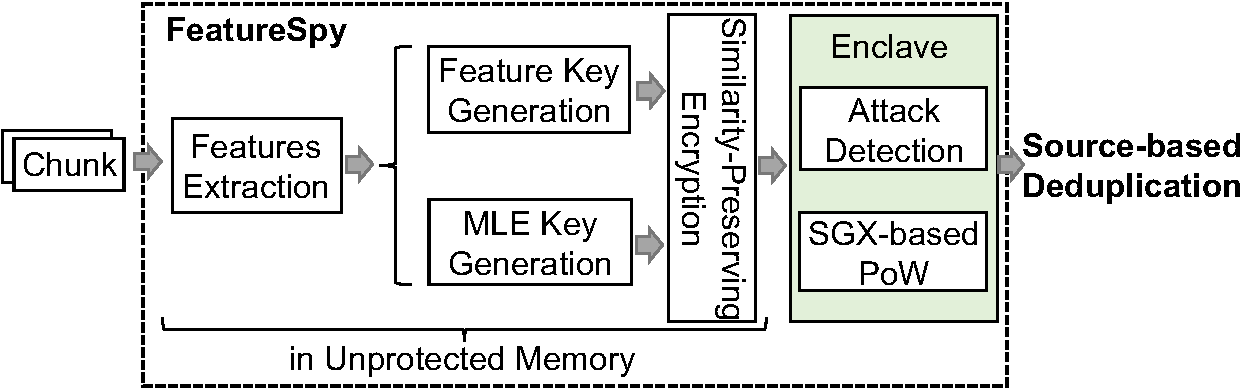
\includegraphics[width=\textwidth]{pic/featurespy/architecture.pdf}
    \caption{基于密文的攻击检测方案工作流程。\sysnameF 将攻击检测程序与安全区中的所有权证明(参见\S\ref{subsec:sgxdedup-arch})结合起来,以恶意客户端防止绕过。}
    \label{fig:featurespy-architecture-secure}
\end{figure}

\sysnameF 提出基于密文数据块的攻击检测方案,并且只将检测过程与安全区中基于TEE的数据所有权证明方案耦合(图~\ref{fig:featurespy-architecture-secure}),以减少可信计算基(TCB)的大小。

\paragraph*{挑战。}
然而,基于密文数据块的相似性检测方案提出了一个新的挑战,因为安全区只能获得加密后数据块,而在消息锁加密之后检测相似性是不可能的。因为消息锁加密密钥从明文数据块(\S\ref{sec:background-enc-deduplication})的全部内容派生加密密钥,使得相似(但不同)的数据块产生不同的加密密钥,进而导致相似的明文数据块被映射到完全不同的密文数据块,使得相似性被破坏。

本文提出一种称为\gls{fbe}的加密原语,它从每个明文数据块的内容特征派生加密密钥(称为特征密钥(Feature key))进行加密/解密操作。由于相似的数据块仅在少数数据区域存在不同,因此它们很可能产生相同的加密密钥。同时,相似数据块(平均大小为8\,KiB)在前几个加密块(在AES中,加密块大小为16字节)相同的概率很高。由于加密重复数据删除\citing{douceur2002reclaiming, shah15}需要使用固定的初始化向量(IV)以保持确定性加密,且链式分组加密模式(Block-chaining encryption,例如\textit{Cipher block chaining (CBC)} 和 \textit{Cipher feedback (CFB)}\citing{dworkin01})的属性使得每个数据块在第一个不同加密块之前的所有加密块均可被加密为相同密文。基于特征的加密保持了明文相似数据块的前几个加密块高概率相同的特性,并且可以通过比较密文数据块前几个加密块是否相同判断对应的两明文数据块是否相似。

然而,基于特征的加密容易受到密钥泄露的影响,因为一个特征密钥对应于一组具有相同内容特征的数据块。恶意客户端可以使用其获得的特征密钥来完全解密多个相似数据块,特别是一些不属于攻击者本身的数据块。

这给加密重复数据删除选择合适的加密原语带来了两难选择:消息锁加密对密钥泄露具有鲁棒性(即,泄露的消息锁加密密钥不能用于解密除相应的数据块之外的其他数据块)但会破坏相似性,而基于特征的加密保留了原始明文数据块的相似性但易受到密钥泄露的威胁。
